\documentclass[10pt,english,a4paper]{article}
\usepackage{graphicx} 
\usepackage{url}
\usepackage{hyperref}

\pagestyle{headings}

\title{Examples of search algorithms used in information retrieval\thanks{Term project in the subject Engineering Methods, ac. year 2023/24, advisor: Ing. Richard Marko, PhD.}}
\author{Jaroslav Ertl\\[2pt]
	{\small Slovak University of Technology in Bratislava}\\
	{\small Faculty of informatics and information technology}\\
	{\small \texttt{xertlj@stuba.sk}}
	}
\date{\small 1. Novemeber 2023} 
\begin{document}

\maketitle
  
\begin{abstract}
    Many people use search engines daily for information retrieval, whether it's for school, work, or personal use, but few understand the complex algorithms that power these systems.  In the realm of Information Retrieval (IR), search algorithms play a crucial role in delivering relevant results from vast datasets. There are many types of search algorithms used in IR, each of them having its unique purpose. 

  You can have a graph-based algorithm, a keyword-based algorithm, and many more. In this article, we will dive into the world of different search algorithms and their application in IR. In each section, we will discuss different search algorithms, how they work, and their purpose.

  You can find the article that guided me towards this topic here \cite{prime_article}.
\end{abstract}
\section{Introduction}
In the digital age, the internet has become a crucial part of our lives, and search engines have become our number one trusted companions. Whether we're seeking answers, writing research for academic purposes or simply satisfying our unending curiosity. But have you ever stopped and thought how that keyword entry turned into relevant results you were seeking? While the act of typing a keyword into a search bar may seem straightforward, beneath the surface lies a world of complexity, driven by search algorithms. 

In this article, we embark on a voyage through the realm of search algorithms. Our first destination on this journey will be the island of graph-based algorithms, where we will delve into the details of Hyperlink-Induced Topic Search (HITS)[section \ref{hits}] and the revolutionary PageRank[section \ref{pagerank}] algorithm. These algorithms have put down the foundation of web search and have transformed the way we discover information online. 

From there, we will set sail for the world of keyword-based algorithms. At this stage of our adventure, we will uncover the mysteries of the Vector Space Model (VSM)[section \ref{vsm}], a mathematical structure that underpins the way documents and queries are represented in the digital space. The VSM allows us to understand how documents are transformed into mathematical vectors and how these vectors are used to determine the relevance of documents to a search query. We will also navigate through the logic of Boolean Search, which includes logical operators to retrieve documents that correspond to our search criteria. And let's not forget the Term Frequency-Inverse Document Frequency (TF-IDF), a cornerstone of keyword-based algorithms. This algorithm has paved the way for innovative approaches in information retrieval. In particular, it laid the foundation for the BM25 search algorithm, which has become one of the most common and influential algorithms used in many search engines today. We will explore the core principles of TF-IDF and how BM25 builds upon this concept to deliver relevant search results to users.
\section{Graph-based algorithms}\label{graph-based}
\subsection{Hyperlink-Induced Topic Search (HITS)}\label{hits}
Our first stop on this journey is an island of Hyperlink-Induced Topic Search(HITS). HITS is an algorithm that is widely used in link analysis. It helps identify webpages across the internet that are related to your specific search. HITS was developed by Jon Kleinberg and is based on the concept that high-quality websites should both link to relevant sites and be linked to by other reliable pages. Imagine the internet as a giant network of interconnected webpages, with each webpage represented as a node and links between them as connections. Some webpages are more important and trustworthy than others, and HITS helps us figure out which ones they are. To understand how this algorithm works and why it is important for us we need to define what authority and hub is. To keep things simple, from now on we will refer to the webpage as a node. Every node is assigned two scores, one for authority and one for hub.
\begin{itemize}
	\item \textbf{Authority} - A node is considered high-quality if many other high-quality nodes refer to it. This essentially means that if trustworthy and valuable nodes on a particular topic link to a specific node, this node is claimed as authoritative for that topic.
	\item \textbf{Hub} - A node is considered as high-quality if it refers to many other high-quality nodes. In other words, if a node links to multiple authoritative nodes, it is seen as a hub, connecting users to valuable information on various topics.
\end{itemize}
For A better understanding of authority and hub, you can take a look at Figure \ref{explanationHITS}. Node 1 has the highest score for hub because it links to the most nodes in this diagram(2 and 4). On the other hand, node 3 has the highest score for authority because it is being linked to by the most nodes(2 and 4).
\begin{figure}[h]
  \centering
  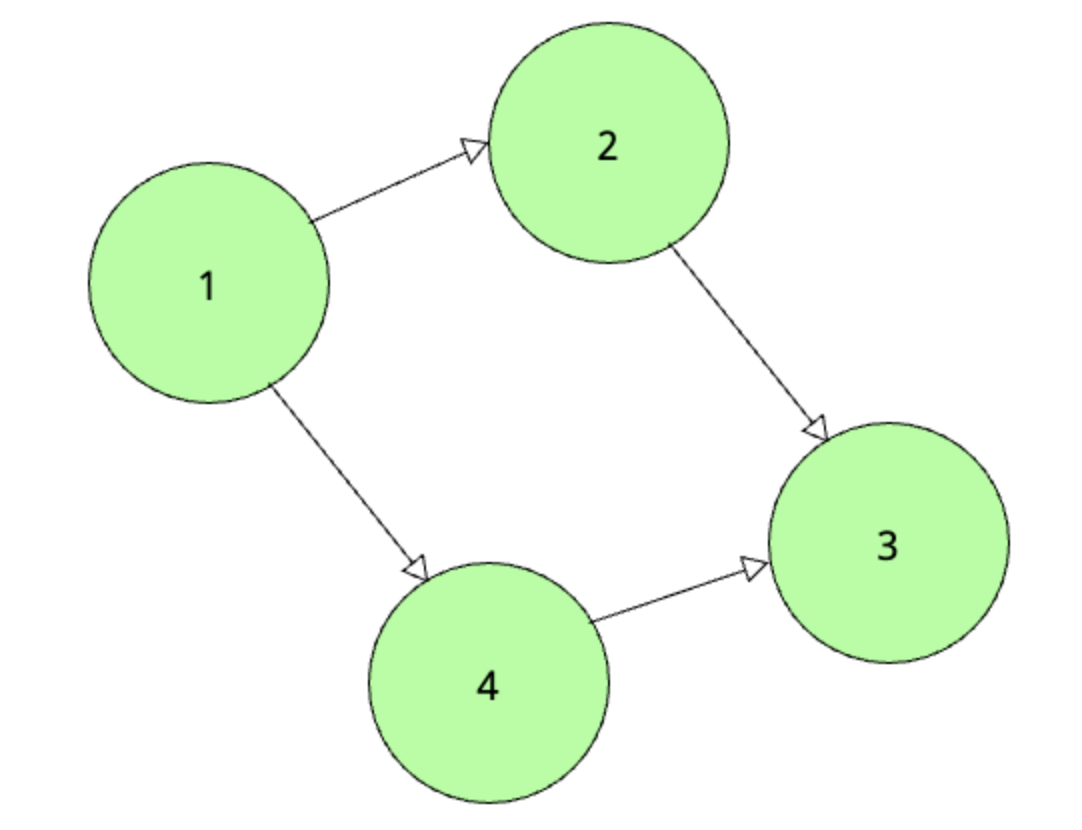
\includegraphics[width=0.5\textwidth]{explanation_HITS.png}
  \caption{Explanation of hub and authority}
  \label{explanationHITS}
\end{figure}
\\\\\\\\
\\Now let's take a look at how the HITS algorithm works:
\begin{enumerate}
  \item \textbf{Initialization} - We start by assigning each node a score for both authority and hub. For simplicity, we often begin with an equal score, typically set to 1.
  \item \textbf{Iteration} - Then we iterate through the nodes updating their authority and hub scores.
  \item \textbf{Updating the score}
  \begin{itemize}
    \item \textbf{Updating the authority} - For the current node, we calculate its authority score by summing the hub scores of all the nodes that link to it. In other words, if several webpages with high hub scores link to the current node, its authority score increases.
    \item \textbf{Updating the hub} - For the current node, we calculate its hub score by summing the authority scores of all the nodes it links to. In other words, if the current connects to authoritative webpages its hub score increases.
  \end{itemize}
  \item \textbf{Repetition} - We repeat this process until the scores no longer change significantly, indicating that we've reached a stable state.
  \item \textbf{Ranking} - The final authority and hub scores are used to rank the nodes. Nodes with higher scores are considered more relevant and trustworthy, allowing us to present users with the most valuable web content.
\end{enumerate} 
It's essential to note that the HITS algorithm's performance can vary depending on the size of the nodes it analyzes. The number of iterations required and the time taken to reach a stable state is strongly influenced by the number of edges and nodes within the network. On a larger scale, more iterations are necessary for the score of each node to stabilize, therefore causing more computation time. 
For instance, consider Figure \ref{comp_time}, which represents a relatively small network consisting of 7 nodes and 18 edges. In this context, the HITS algorithm would require approximately 5 iterations to reach a stable state. The computation time in such a scenario is relatively short. However, in contrast, imagine a bigger network with 1000 nodes and 5000 edges. Even after 500 iterations of the HITS algorithm, this larger network might still not have reached a stable state due to its complexity.
\begin{figure}[h]
  \centering
  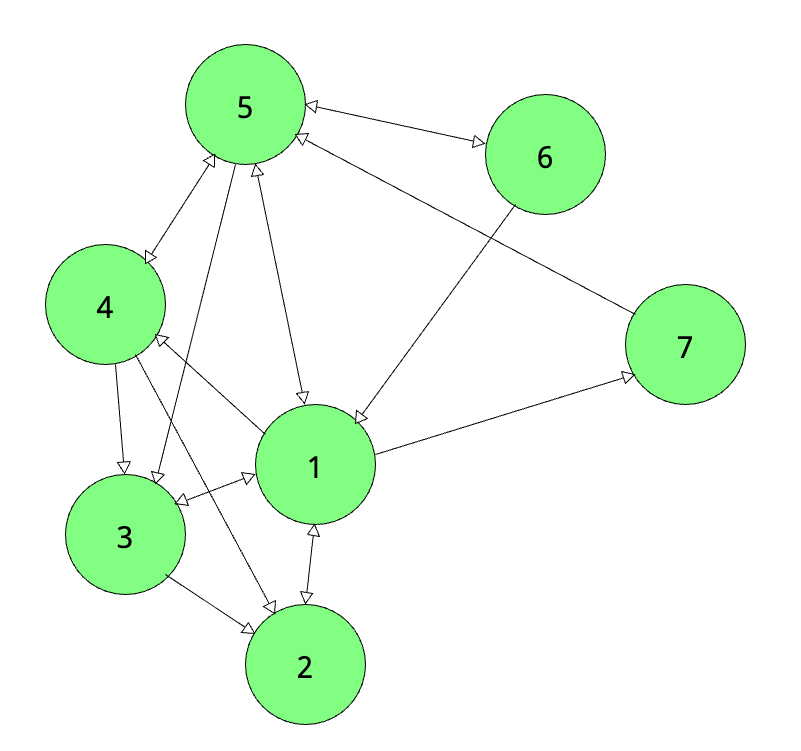
\includegraphics[width=0.5\textwidth]{comp_time_1.png}
  \caption{Iteration time example by T.Chou\cite{hits_article}}
  \label{comp_time}
\end{figure}

Although HITS is playing significant role in information retrieval and in improvements of search engines, it has some challenges associated with itself.
\begin{itemize}
  \item \textbf{Low Computational Efficiency} - As we have already mentioned, the HITS algorithm's computation efficiency varies depending on the size of the network and the data it works with. When working with huge amounts of data it can take vast amount of time to complete the results.
  \item \textbf{Results Can Be Manipulated} - The HITS algorithm is vulnerable by cheaters. For instance, a cheater can build a website that links to other high-quality websites, this website then gets a good hub score. Then the cheater allows this website link to his own website. This way he can increase the authority score of his website.  
\end{itemize}
Yet, despite these challenges, the HITS algorithm remains a foundation tool in the realm of information retrieval, helping us to find relevant information on the web with precision and accuracy.\cite{hits_challenges_article}
\subsection{PageRank}\label{pagerank}
As we continue to sail through, our next destination is the fascinating PageRank algorithm. Created by Google, PageRank acts as a beacon that shows a path for us towards the most valuable websites. What sets the PageRank apart from HITS is that the PageRank is query-independent, which simply means that it doesn't rely on the specific content or keywords of a user's search query to determine the result. Instead, it focuses on the web's link structure. It carefully counts the number and quality of links leading to a website, offering a rough estimate of the quality of the website. The assumption is that high-quality websites tend to receive more connections from other webpages across the internet.

The steps of this algorithm are similar to the ones that we have already seen in the HITS algorithm. Let's take a better look at them:
\begin{enumerate}
  \item \textbf{Initialization} - PageRank scores are assigned to each webpage, typically starting with an equal score, often set to 1, to treat all pages equally and initiate the process.
  \item \textbf{Redistribution} - During each iteration, PageRank redistributes scores based on the links between webpages. The more outbound links a webpage has, the more its PageRank is divided among those links.
  \item \textbf{Damping factor} - PageRank introduces a damping factor, typically set around 0.85. This factor simulates the probability that a user might randomly jump to any webpage rather than following links, adding a layer of realism to the calculations.
  \item \textbf{Repetition} - These steps and calculations are repeated for all webpages in the network until the PageRank scores no longer change significantly.
  \item \textbf{Ranking} -  After a sufficient number of iterations, the PageRank scores are used to rank webpages. Webpages with higher scores are considered more relevant and trustworthy, playing a crucial role in search engine ranking and information retrieval.
\end{enumerate}
You can represent PageRank as a mathematical equation as well. The equation is shown below
\[
PR(p_i) = \frac{1 - d}{N} + d \sum_{p_j \in M_{p_i}} \frac{PR(p_j)}{L(p_j)} \quad {\cite{pageRank_formula_article}}
\]
where $PR(p_i)$ and $PR(p_j)$ represents the influence of node $p_i$ and $p_j$. The parameter $d$ represents the damping factor, $N$ represents the number of all nodes in the network. $M_{p_i}$ represents the set of nodes that link to $p_i$ and $L(p_j)$ represents the set of nodes that link to $p_j$. 
\begin{figure}[h]
  \centering
  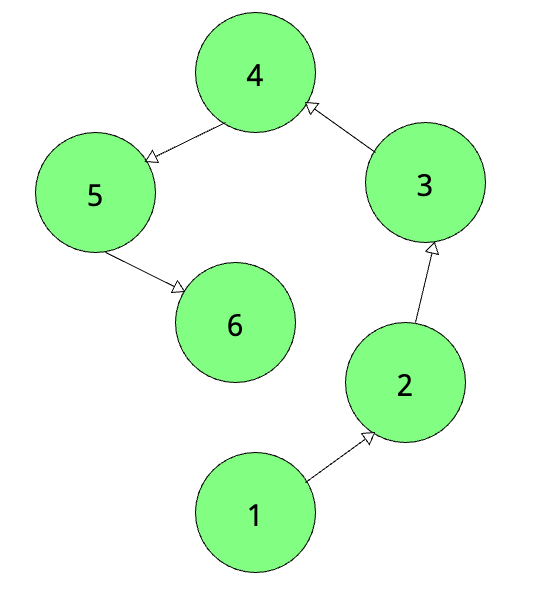
\includegraphics[width=0.45\textwidth]{explanation_PageRank.png}
  \caption{PageRank example by T.Chou\cite{pageRank_article}}
  \label{explanation_PageRank}
\end{figure}

For a better understanding of PageRank, let's take a look at Figure \ref{explanation_PageRank}. In this example, we have 6 nodes each with a score of 1 at the start. Then we proceed with the algorithm steps. After each iteration, score of each node recalculates. The reason the scores change in each iteration is due to the flow of PageRank between nodes. This means that node 2 will receive a rank from node 1, node 3 will receive a rank from node 2, and so on. Here damping factor plays a significant role, it ensures that not all PageRank from a previous node is passed to the next node. After a few iterations, we would enter a stable state where node 6 would have the highest PageRank with a score of \textit{0.252}, thanks to receiving the PageRank from nodes 1 to 5. On the other hand, node 1 would have the lowest PageRank with a score of \textit{0.061}.

In conclusion, the PageRank algorithm has fundamentally shifted the way we navigate and retrieve information on the web. While PageRank has revolutionized web search, it wasn't an easy path without any challenges to face. It has similar efficiency to the HITS algorithm when it comes to bigger networks. It can be manipulated through tactics such as link farming, which is uniform to the HITS algorithm. Nevertheless, it remains a crucial component in our journey through the world of search algorithms.
\section{Keyword-based algorithms}
\subsection{Boolean Search}\label{boolean_search}
Now, that we've abandoned the world of graph-based algorithms, let us explore the possibilities of keyword-based algorithms. Starting with none other than Boolean Search. It is known that when the user is typing a query, usually consisting of one or more words, he needs to choose his words precisely. The system then determines which documents are the most relevant to the query. Instead of leaving this decision solely to the system, users can play a crucial role in this by choosing precise query expressions using a set of operators.  This technique is called Boolean Search. The Boolean retrieval model for information retrieval revolves around formulating queries in the form of Boolean expressions, combining terms with operators like AND, OR, and NOT. In this model, each document is treated as a collection of words, allowing for systematic and targeted information retrieval \cite{boolean_search_article}.
%TODO add more info about boolean search

\subsection{Vector Space Model}\label{vsm}
Next stop on our journey will be the Vector Space Model (VSM).Composed by G. Salton, VSM stands as one of many models used in information retrieval. Its basic thought is that it transforms the unending content of text documents and user queries into one point in multidimensional space, and is thought of as a vector\cite{VSM_explanation_article}. This transformation opens the door to calculating similarity with breathtaking precision, making VSM an invaluable tool for various applications. 

In the Vector Space Model (VSM), every document is represented as a vector in a multi-dimensional space, with each document consisting of terms denoted as $T_1, T_2, T_3, \ldots, T_n$. These terms are considered independent, and each term ($T_i$) is assigned a weight ($W_i$) that reflects its importance within the document. Think of these terms as coordinate axes in an N-dimensional space and the assigned weight as the value associated with each axis\cite{VSM_weight_terms_article}. The determination of these weights is typically accomplished using the TF-IDF (Term Frequency-Inverse Document Frequency) scheme[\ref{tf-idf}].

Additionally, some VSM implementations may involve a feature selection process. This process aims to select a subset of terms from the original set of terms. The ultimate goal of feature selection is to enhance the computation of document similarity. The selected features should be indicative of the document's theme and relevance to user queries\cite{VSM_weight_terms_article}.
It's important to note that the feature selection step is not always included in every VSM implementation, and its inclusion depends on specific requirements and objectives.
%TODO explain practical uses and challenges
\subsection{TF-IDF}\label{tf-idf}
\section{Conclusion}
\section{Lectures}
\bibliographystyle{unsrt} 
\bibliography{literatura}
\end{document}
